\documentclass[t,10pt]{beamer}
\usetheme[official=true,titlebgimage=toro,conference=\mbox{N. Vianello
  @ KTH 22 June 2011}]{rfx}
\usepackage[english]{babel}
\usepackage{listings,amsmath,multimedia}
\usepackage{tangocolors}
\usepackage{rfxcolor}
\usepackage{pgf}
\usepackage{tikz}
\usepackage[bibstyle=numeric-comp,citestyle=authoryear-comp,labelyear=true,maxnames=1]{biblatex}
\bibliography{biblio}
\renewcommand*{\bibfont}{\footnotesize}
\mode<presentation>
\graphicspath{{pdf_box/}}
\renewcommand\Re{\operatorname{Re}}
\renewcommand\Im{\operatorname{Im}}

% for adding foot note with reference
\makeatletter
% add a macro that saves its argument
\newcommand{\footlineextra}[1]{\gdef\insertfootlineextra{#1}}
\newbox\footlineextrabox

% add a beamer template that sets the saved argument in a box.
% The * means that the beamer font and color "footline extra" are automatically added. 
\defbeamertemplate*{footline extra}{default}{
    \begin{beamercolorbox}[ht=2.25ex,dp=1ex,leftskip=\Gm@lmargin]{footline extra}
    \insertfootlineextra
    %\par\vspace{2.5pt}
    \end{beamercolorbox}
}

\addtobeamertemplate{footline}{%
    % set the box with the extra footline material but make it add no vertical space
    \setbox\footlineextrabox=\vbox{\usebeamertemplate*{footline extra}}
    \vskip -\ht\footlineextrabox
    \vskip -\dp\footlineextrabox
    \box\footlineextrabox%
}
{}

% patch \begin{frame} to reset the footline extra material
\let\beamer@original@frame=\frame
\def\frame{\gdef\insertfootlineextra{}\beamer@original@frame}
\footlineextra{}
\makeatother

\setbeamercolor{footline extra}{fg=structure.fg}% for instance

\title{Research \& Pedagocical activity \\
{\small Status and Plans}}
\author{N. Vianello }
\date{22 June 2011}

\begin{document}

\begin{titleframe}
\end{titleframe}

\begin{frame}{Personal research interest}
\begin{itemize}
{\large\item The candidate has been active in fusion plasma physics since the
M.Sci. thesis in 1999
\item Personal research interests can be described in three main
  macro-areas
\begin{description}
\item[(A)] \textcolor{taorange}{Turbulence \& Flows in magnetized plasmas}
\item[(B)] \textcolor{ta3skyblue}{Statistical characterization of
    electromagnetic fluctuations}
\item[(C)]\textcolor{ta3chameleon}{Emerging of electromagnetic structures}
\item[(D)] \textcolor{tascarletred}{Spontaneously developed Helical plasmas}
\end{description}
}\end{itemize}
\end{frame}

\begin{frame}{Turbulence \& Flows}


%% per aggiungere la lettera colorata con l'argomento in alto a sx'
\begin{tikzpicture}[remember picture, overlay]
\node [shift={(-0.779 cm,-0.3cm)}]  at (current page.north east)
   {\tikz[baseline=(t1.base)]{\node[fill=taorange](t1){%
{\large A}};}
    };
\end{tikzpicture}
%%
\begin{itemize}
\item The principal results may be summarized as follows:
\begin{columns}
\onslide<2->{\begin{column}{0.48\textwidth}
\begin{block}{}
(i) Role of electrostatic Reynolds stress in momentum generation in RFPs
\end{block}
\begin{center}
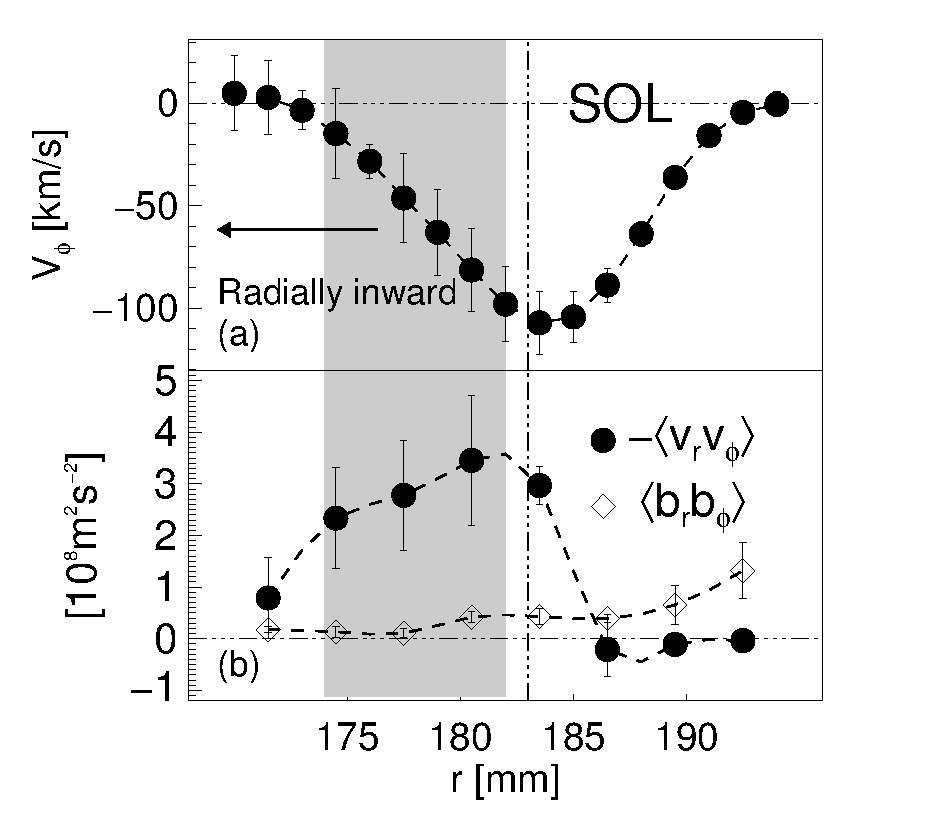
\includegraphics[height=3.8cm]{Profili-Rs-velocity} \\
{\tiny PRL 94 p. 135001, NF 45 p. 761, PPCF 48 p. S193}
\end{center}
\end{column}
}
\onslide<3>{\begin{column}{0.48\textwidth}
\begin{block}{}
(ii) Transport reduction induced by active modification of
  sheared flow
\end{block}

\vspace{.36cm}

\begin{center}
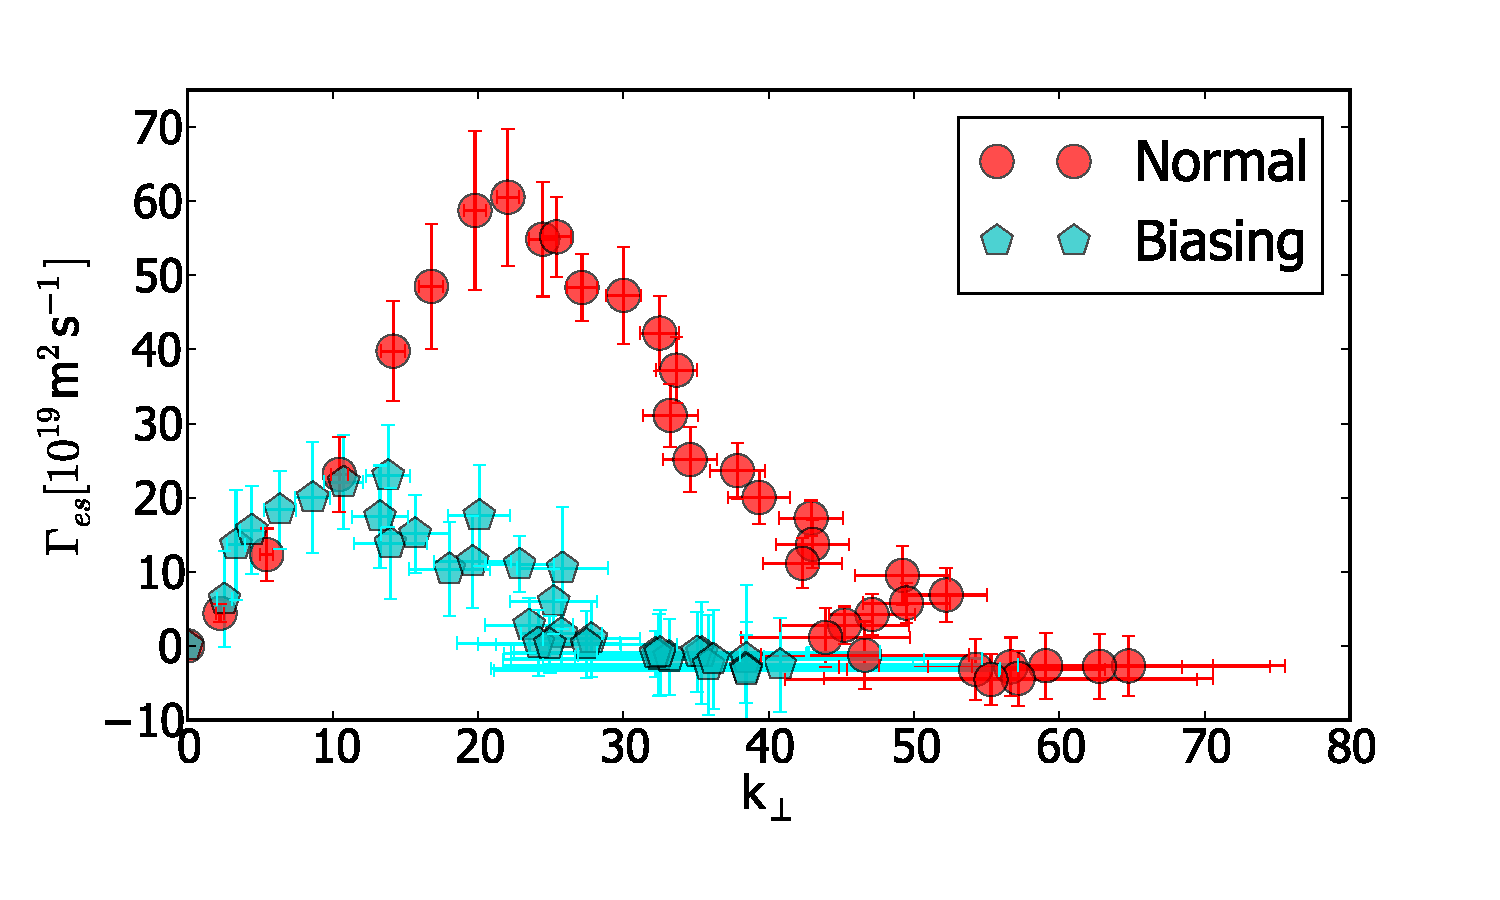
\includegraphics[height=3.4cm]{flux_biasing} \\
{\tiny PPCF 42, p. 83}
\end{center}
\end{column}
}
\end{columns}
\end{itemize}
\end{frame}


\begin{frame}{Intermittency \& SOC}
%% per aggiungere la lettera colorata con l'argomento in alto a sx'
\begin{tikzpicture}[remember picture, overlay]
\node [shift={(-0.779 cm,-0.3cm)}]  at (current page.north east)
   {\tikz[baseline=(t1.base)]{\node[fill=ta3skyblue](t1){%
{\large B}};}
    };
\end{tikzpicture}
%%
\begin{itemize}[<+->]
\item The presence of
  \textcolor{ta3chameleon}{\texttt{Intermittency}}, as lack of
  self-similarity, revealed in laboratory plasmas, in analogy to solar
  wind turbulence and ordinary flow

\begin{center}
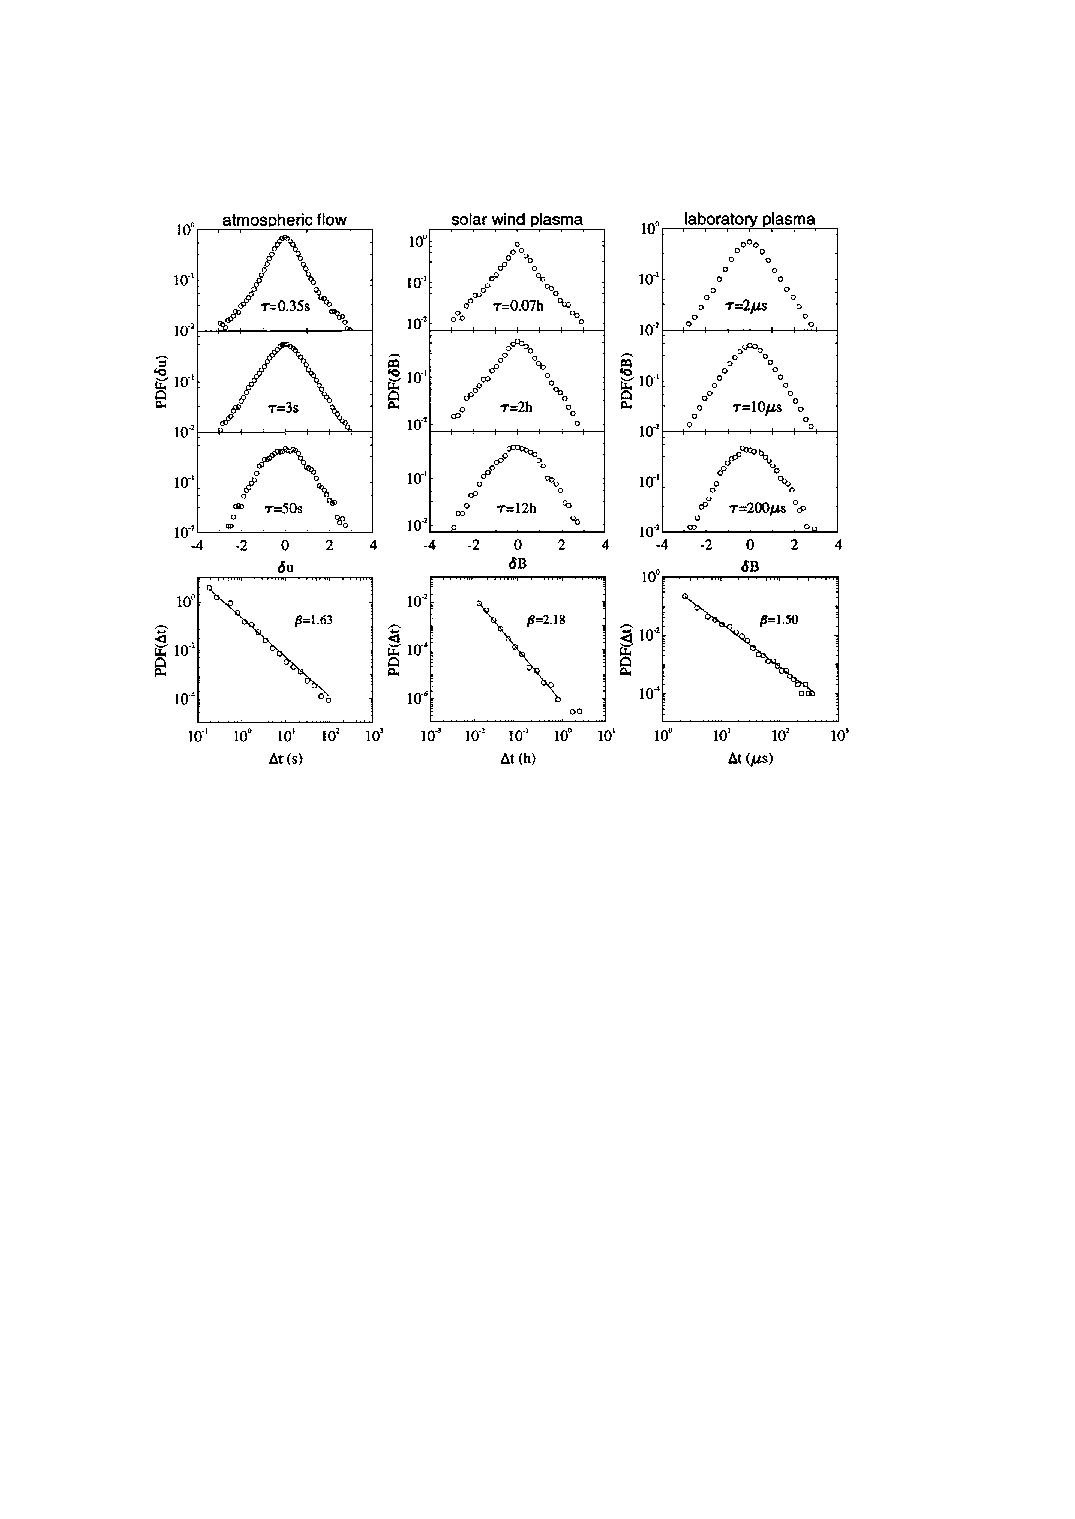
\includegraphics[height=5.2cm]{global-intermittency} \\
{\tiny EPL 54 p.51, PRL 87 p.045001, PPCF 2002 pp 2513, EPL 58, pp 349 }
\end{center}

\item Inconsistency with
  \textcolor{ta3chameleon}{\texttt{SOC}} model revealed
{\tiny PRL 86 pp 3032, EPL 58 pp 349, PRL 87 045001 }
\end{itemize}
\end{frame}


\begin{frame}{Coherent structures characterization}
%% per aggiungere la lettera colorata con l'argomento in alto a sx'
\begin{tikzpicture}[remember picture, overlay]
\node [shift={(-0.779 cm,-0.3cm)}]  at (current page.north east)
   {\tikz[baseline=(t1.base)]{\node[fill=ta3chameleon](t1){%
{\large C}};}
    };
\end{tikzpicture}
%%


\begin{columns}[t]
\begin{column}{0.47\textwidth}
\begin{itemize}
\item Complete characterization of coherent structures responsible for
  intermittency 
\begin{center}
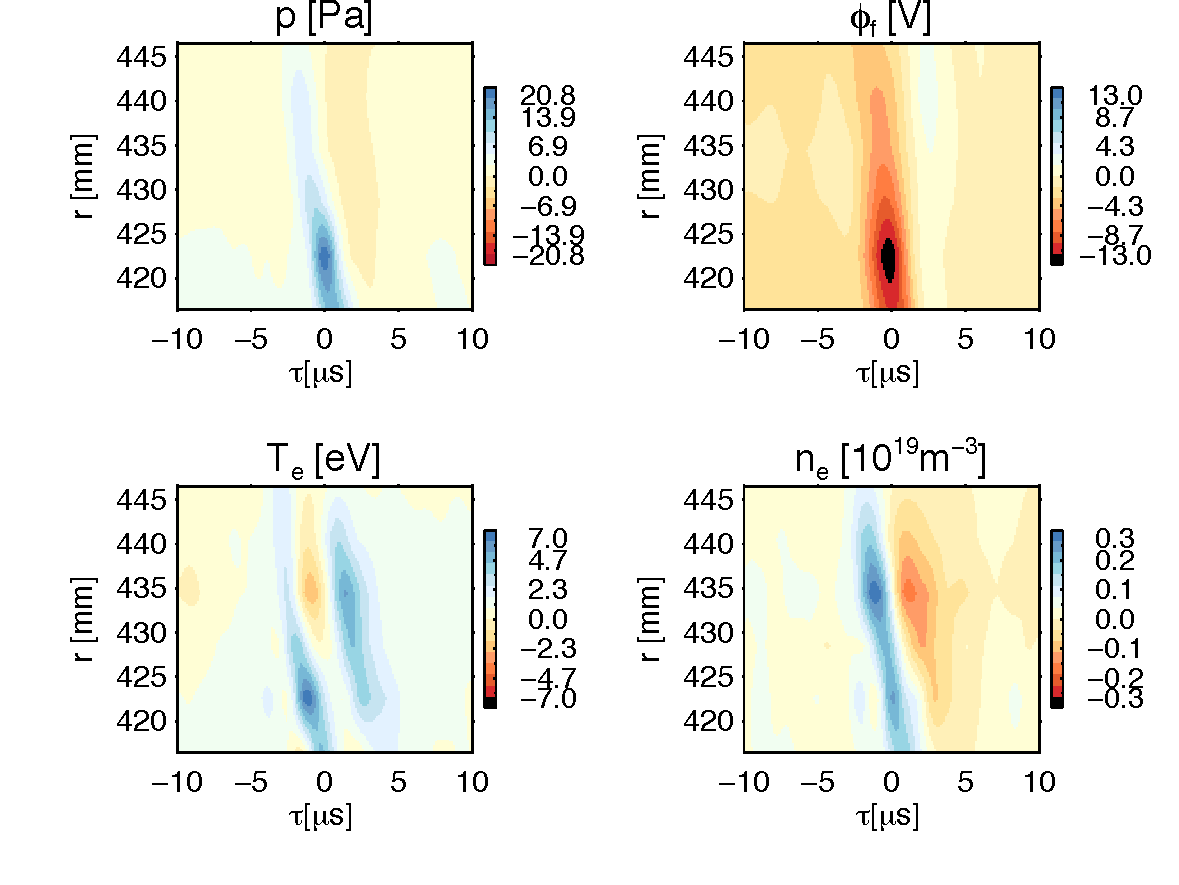
\includegraphics[height=4.5cm]{2Dstructure}
\end{center}
\end{itemize}
\end{column}
\pause
\begin{column}{0.5\textwidth}
\begin{itemize}
\item Evaluation of transport contribution due to coherent structures
\end{itemize}
\begin{center}
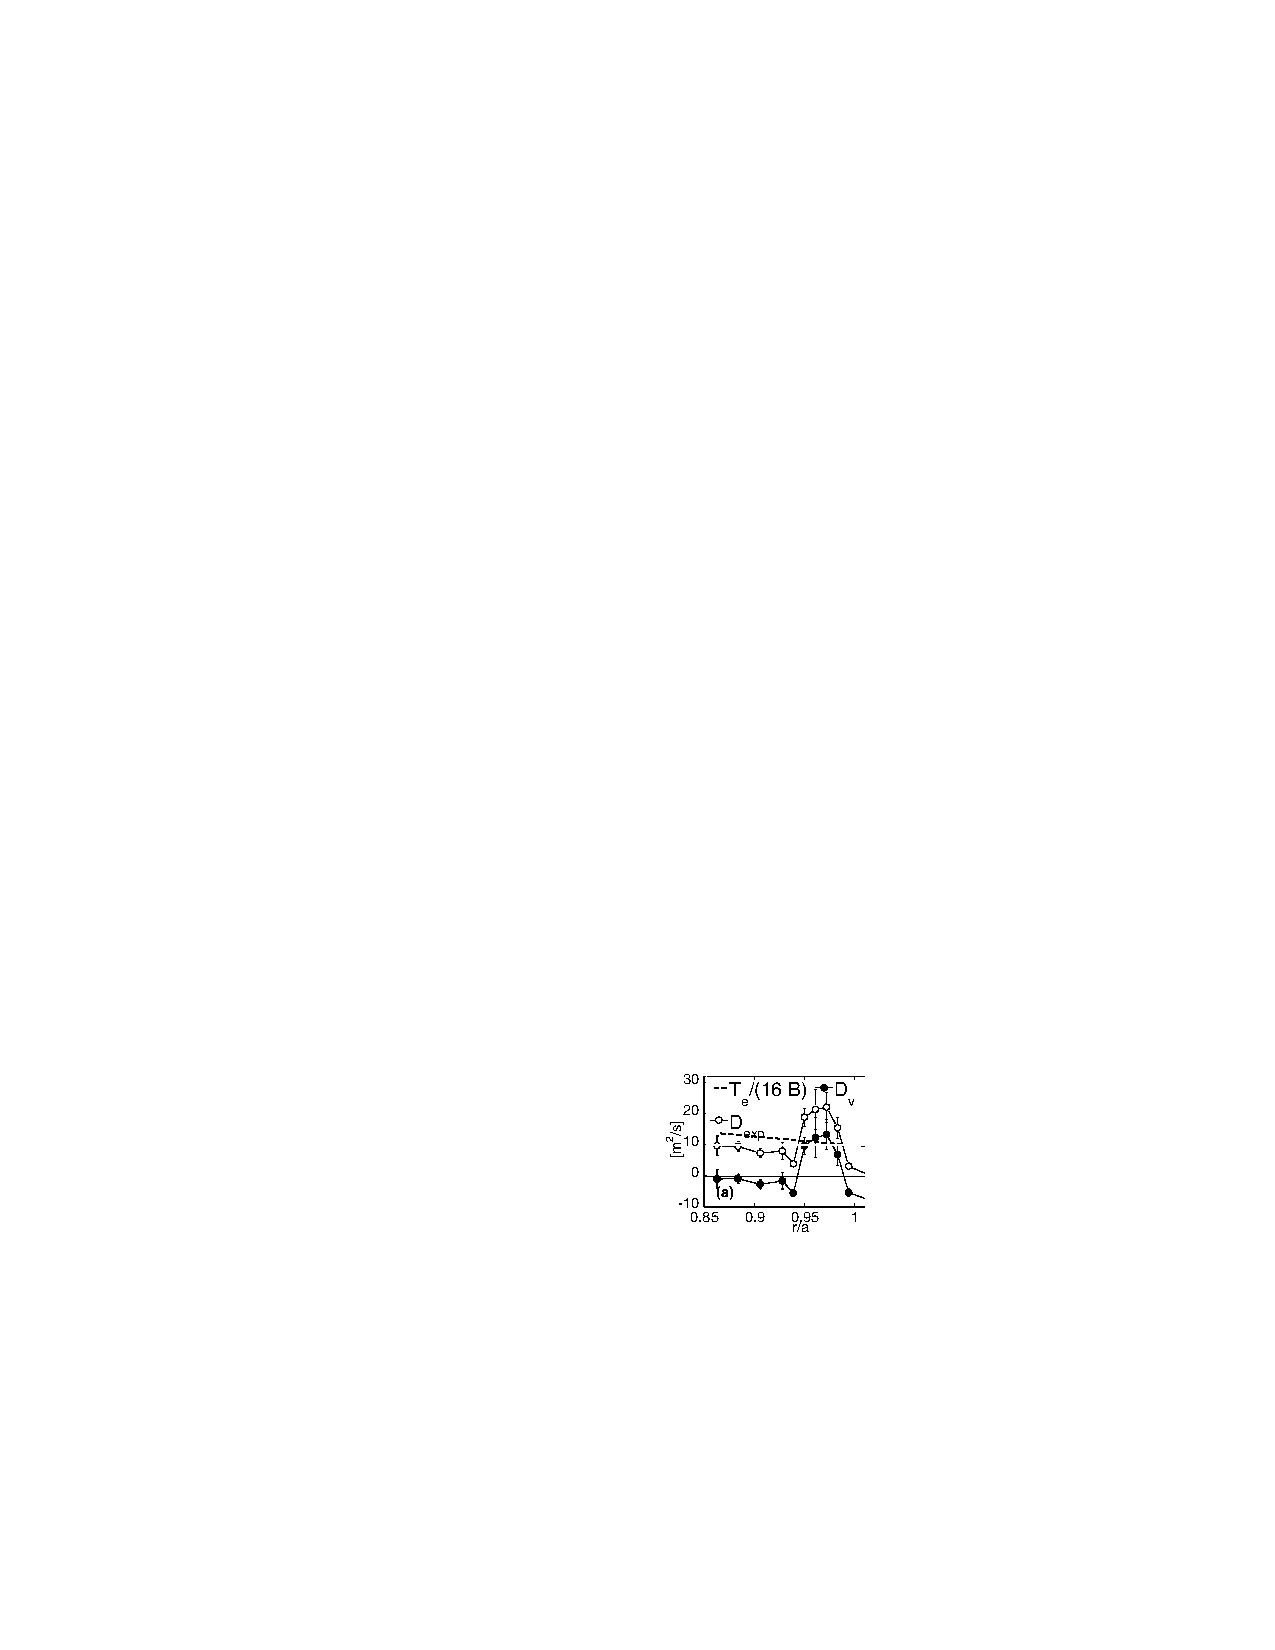
\includegraphics[height=3cm]{structure-diffusivity}
\end{center}
\end{column}
\end{columns}
\begin{center}
{\tiny PRL 93 p.215003, PoP 9 p.4110}
\end{center}
\end{frame}
\begin{frame}{Current filaments}
%% per aggiungere la lettera colorata con l'argomento in alto a sx'
\begin{tikzpicture}[remember picture, overlay]
\node [shift={(-0.779 cm,-0.3cm)}]  at (current page.north east)
   {\tikz[baseline=(t1.base)]{\node[fill=ta3chameleon](t1){%
{\large C}};}
    };
\end{tikzpicture}
%%
\begin{itemize}
\item {\small Measurements of parallel plasma current associated to
  \emph{blobs} \& \emph{filaments} in different experiments}
\begin{center}
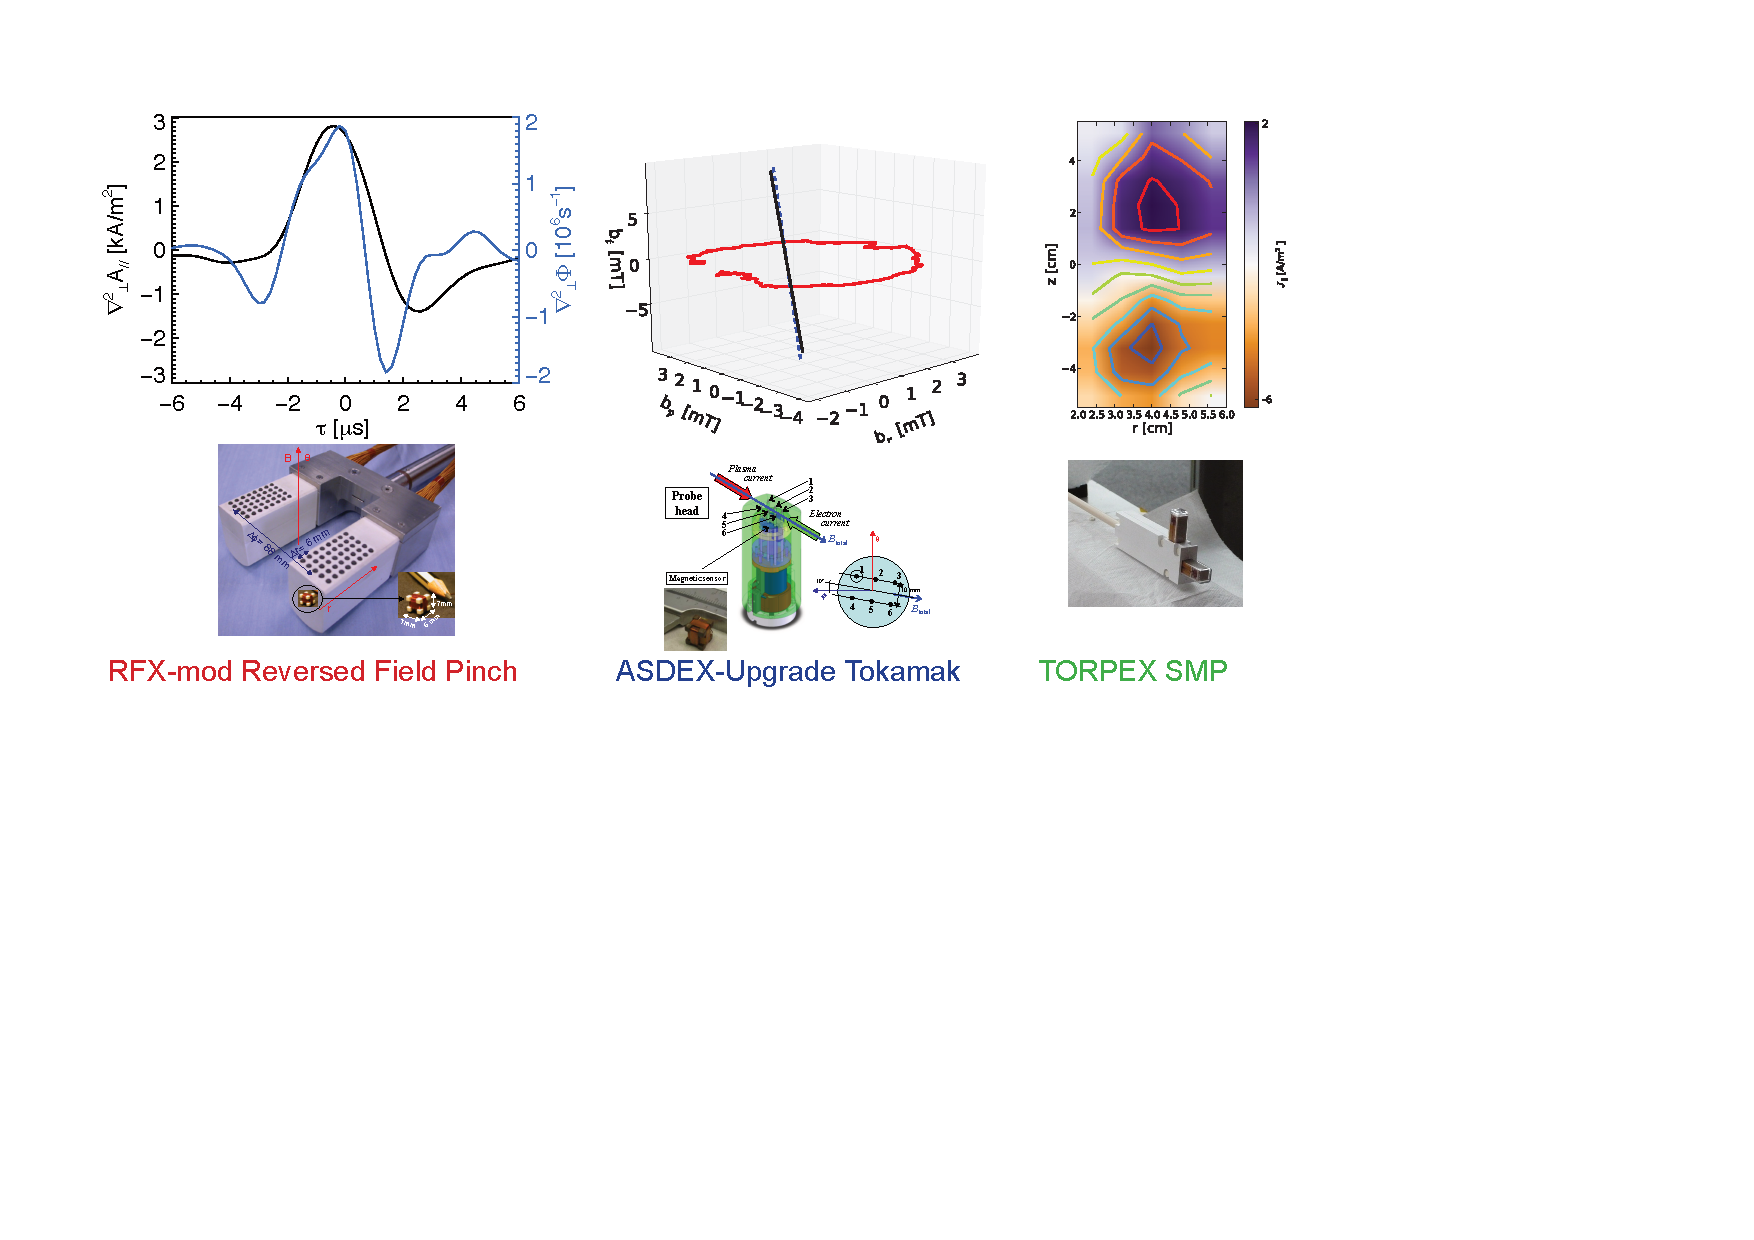
\includegraphics[width=0.78\textwidth]{all-currents}
\end{center}

\item {\small Parallel current measured for
  \textcolor{ta3scarletred}{\texttt{Drift-Kinetic Alfv\'en vortices}}
  in RFX-mod {\tiny (PRL 102 p 165001, NF 50 p.042002)},
  \textcolor{ta3skyblue}{\texttt{type I ELMs  filaments}} in ASDEX-Upgrade {\tiny (PRL 106 p 125002)}, 
  \textcolor{ta3chameleon}{\texttt{interchange-induced blobs }} in TORPEX (CRPP) {\tiny (PRL 106 p 245001)}}
\end{itemize}
\end{frame}
\begin{frame}{Current filaments}
%% per aggiungere la lettera colorata con l'argomento in alto a sx'
\begin{tikzpicture}[remember picture, overlay]
\node [shift={(-0.779 cm,-0.3cm)}]  at (current page.north east)
   {\tikz[baseline=(t1.base)]{\node[fill=ta3chameleon](t1){%
{\large C}};}
    };
\end{tikzpicture}
%%
\begin{itemize}
\item Collaboration established to extend studies of current filaments
  to other devices, namely \textcolor{ta3chameleon}{\texttt{TJ-II
      stellarator}}, with a probe which combines vorticity and current
  measurements and \textcolor{ta3skyblue}{\texttt{EAST tokamak}} for
  the studies of ELMs
\begin{center}
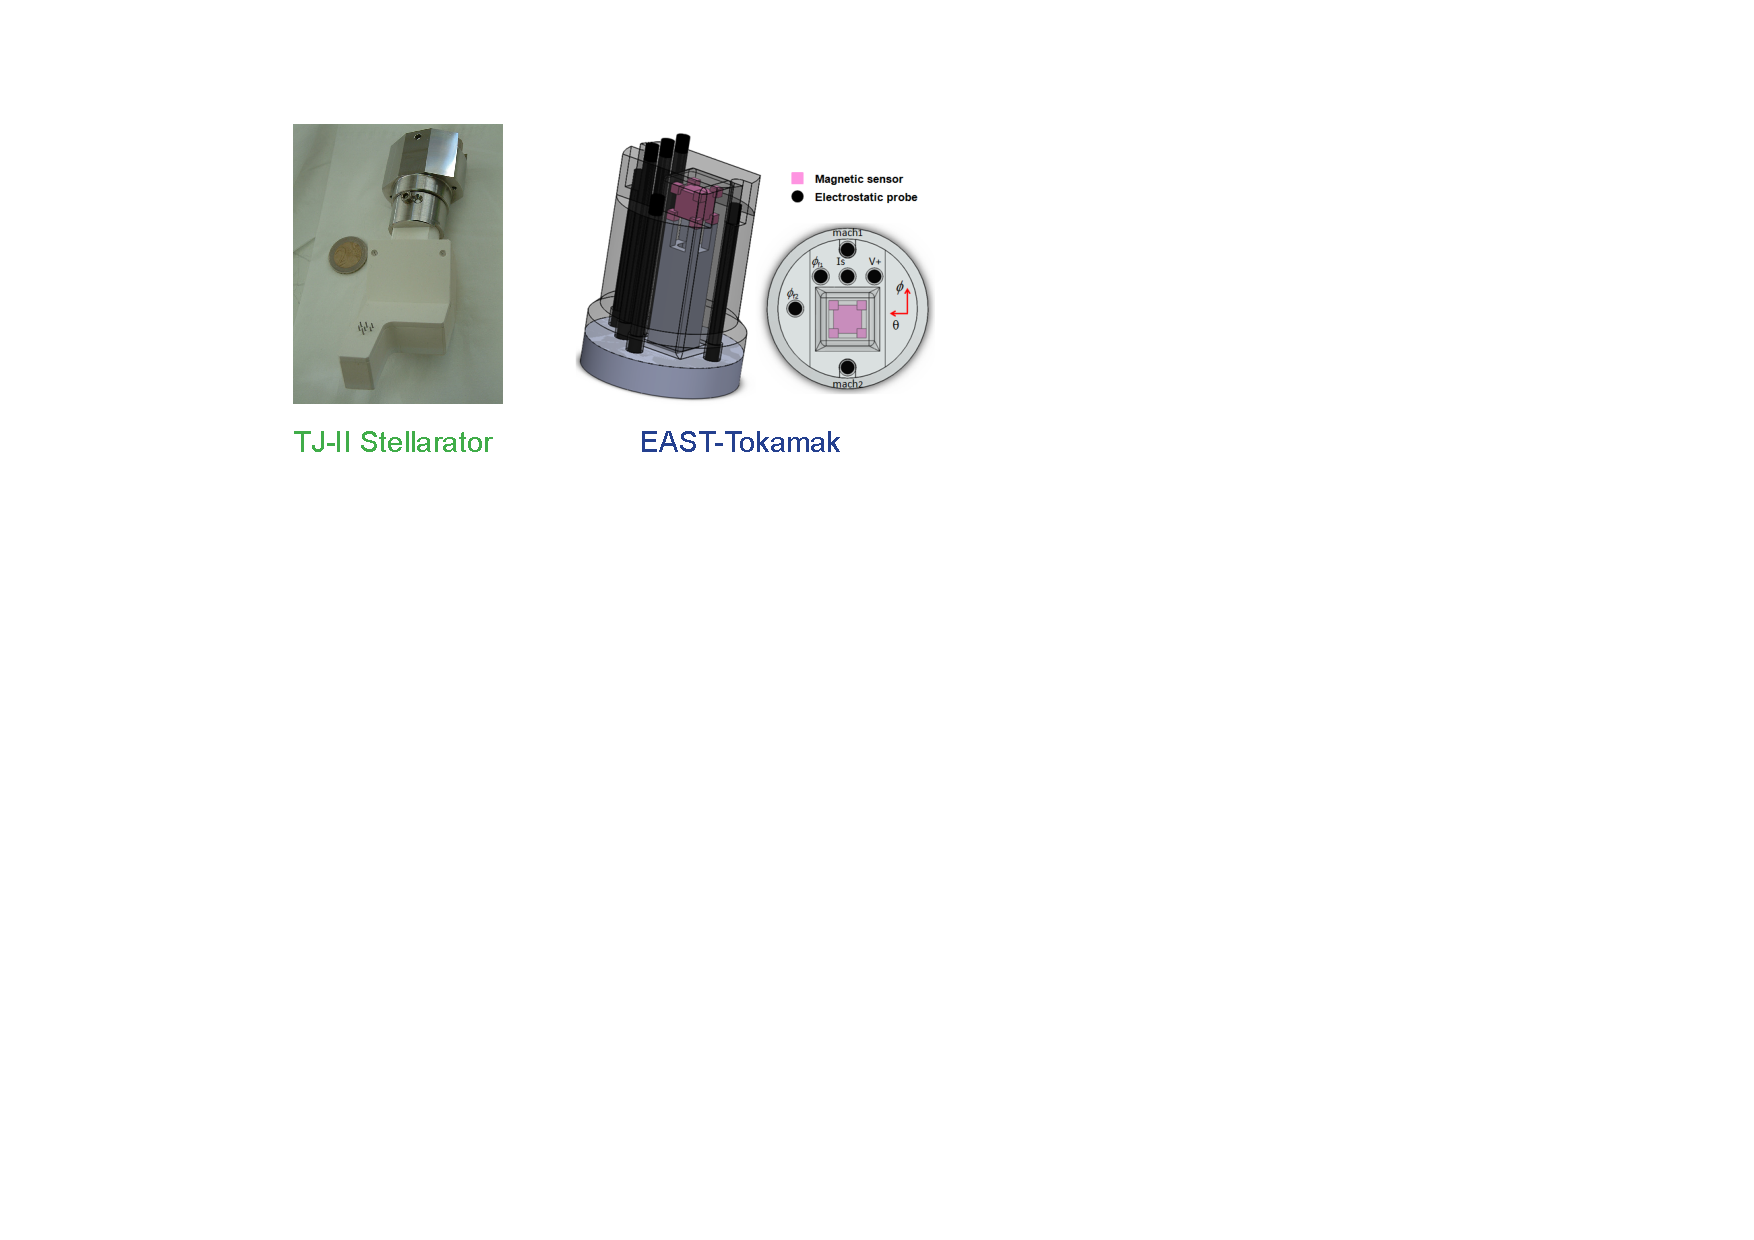
\includegraphics[height=4cm]{collaboration}
\end{center}
\item Coordination of EFDA working group on 3D field effects in edge
  and SOL and diagnostic development under EFDA Transport Topical
  Group for 2011
\end{itemize}
\end{frame}


\begin{frame}{Helical plasmas}
%% per aggiungere la lettera colorata con l'argomento in alto a sx'
\begin{tikzpicture}[remember picture, overlay]
\node [shift={(-0.779 cm,-0.3cm)}]  at (current page.north east)
   {\tikz[baseline=(t1.base)]{\node[fill=tascarletred](t1){%
{\large D}};}
    };
\end{tikzpicture}
%%
\only<1>{\vspace{1cm}

\begin{columns}[c]
\begin{column}{0.4\textwidth}
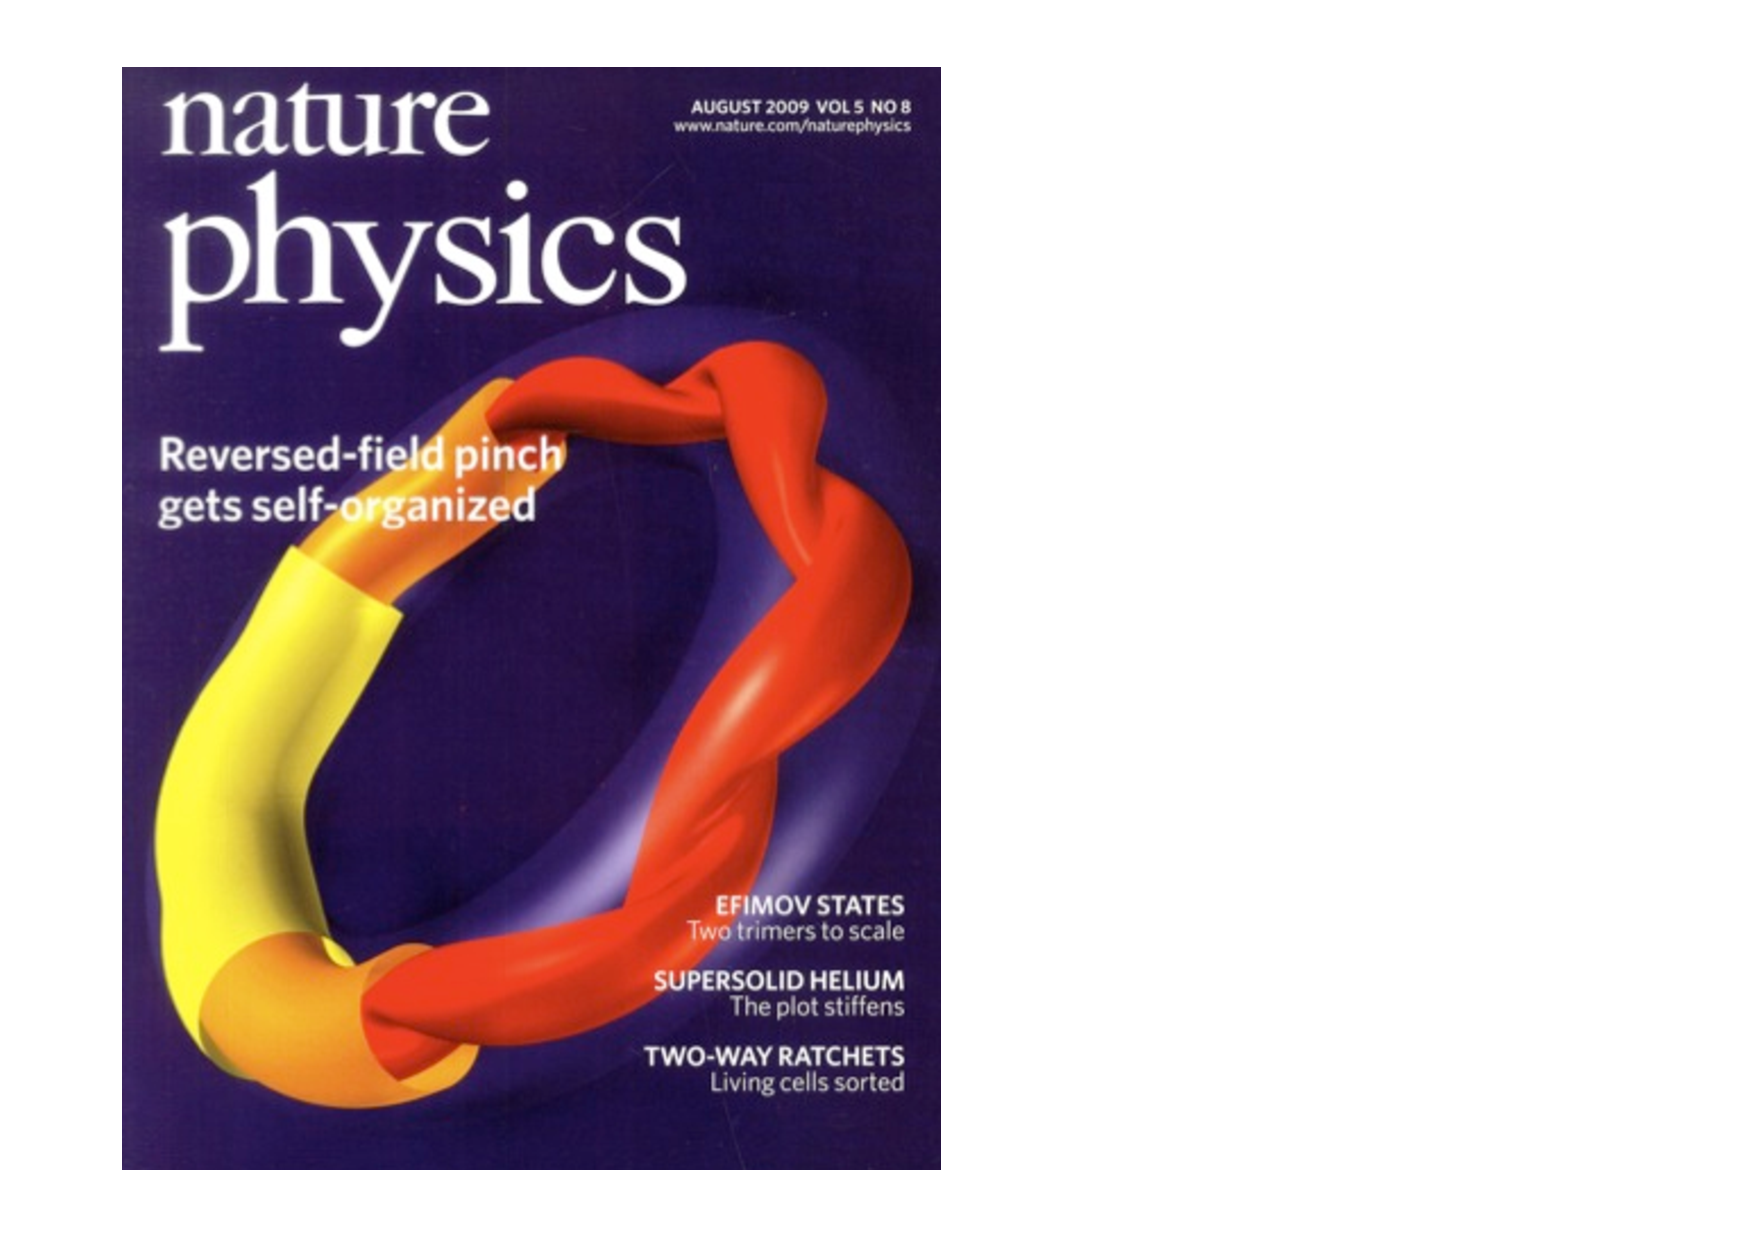
\includegraphics[height=5cm]{copertina}
\end{column}
\begin{column}{0.58\textwidth}
\begin{itemize}
\item {\large Observation and characterization of spontaneous helical plasmas
  developing in high current Reversed Field Pinch operation {\small
    Nat. Phys. 5 pp. 570}}
\end{itemize}
\end{column}
\end{columns}
}
\only<2>{

\begin{center}
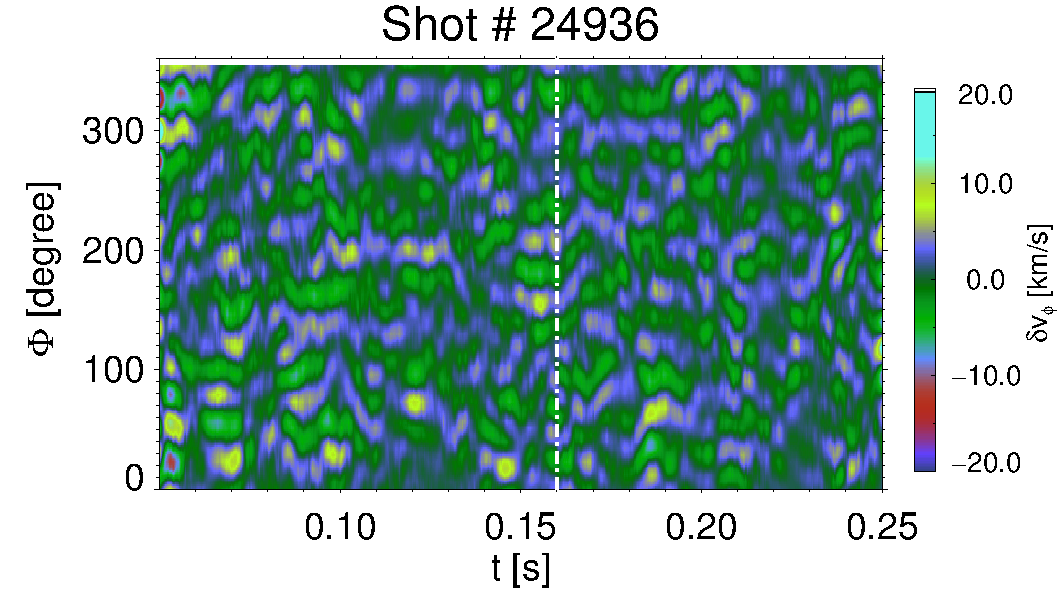
\includegraphics[width=7.cm]{helical-flow}
\end{center}
\begin{itemize}
\item Small residual helical ripple influence on edge physics
\item Helical flow associated to dominant mode
\item Relationship between magnetic topology and flow also in the
  framework of high density radiative collapse
\end{itemize}
\begin{center}
{\tiny PPCF 52, pp 095011, CPP 50 pp. 824, NF 51, 073002}
\end{center}
}
\end{frame}

\begin{frame}{Pedagogical experience}
\begin{itemize}
\item Assistant for the course \textcolor{ta3chameleon}{\texttt{Fluid and Plasma physics} }with
  lessons on \textcolor{ta3chameleon}{\texttt{Tangential stress in a newtonian fluid}} and
  exercise on fluid dynamics
\item Supervising of 2 Bachelor Thesis and 1 Ms.Sci. Thesis on Plasma
  physics. Addressed the following thematic:
\begin{description}
\item[(a)] BA.: Modification of spectral properties of fluctuations as a
  function of plasma equilibria in a Reversed Field Pinch. Role on the
  emphasis of $m=0$ islands
\item[(b)] BA: The role of toroidal flow in the high density regimes
  of an RFP plasma. Relation between flow and topology
\item[(c)] M.Sci: Comparison between filamentary structures in a
  Reversed Field Pinch and a Tokamak
\end{description}
\end{itemize}
\end{frame}

\begin{frame}{Planned research activity}
\begin{description}
\item[3D effects on flow and transport:] 3D effects are
  present in almost all the present experiment and foreseen for future
  one. The role of 3D magnetic field on flow, both in the external
  region where stochastic layer can be created, and in the core are
  fundamental topic to be addressed and considered
\item[Fast ions:] MHD and turbulence modification of fast ion
  population is a subject to be investigated for future
  machines. Experimentally, small devices may be thought as test bed
  if equipped with tools for fast ion injections (Beam or ion
  sources), or if available spontaneous population (reconnecting processes)
\item[Spontaneous magnetic reconnection:] Interdisciplinary subject
  where collaboration with space and astrophysical plasma may be considered 
\end{description}
\end{frame}

\begin{frame}{Planned pedagogical activity}
\begin{description}
{\large \item[Multidisciplinary approach to data analysis:] A lot of
  techniques, used in different research area (e.g. space plasma,
  signal and image processing etc.), may be applied to
  fusion plasma data}
{\large\item[Small fusion device as learning tools:] The use of smaller
  device, eventually with cold plasmas may offer the opportunity
  for students for a comprehensive approach to the data, from the
  diagnostic through the acquisition up to the analysis }
\end{description}
\end{frame}

\end{document}
